\section{Auswertung}
Die Auswertung, genauer die Fehlerrechnung, die Plots und Ausgleichsrechnung erfolgt mit den Paketen
Numpy \cite{numpy}, Uncertainties \cite{uncertainties}, Matplotlib \cite{matplotlib} und Scipy \cite{scipy} in der Programmiersprache python.
\subsection{Fehlerrechnung}
Die Mittelwerte werden nach
\begin{equation}
	\bar{x}=\frac{1}{N}\sum_{i}^N x_i
\end{equation}
und deren Standardabweichung mit
\begin{equation}
	\sigma_{\bar{x}} = \sqrt{\frac{1}{N(N-1)} \sum_{i}^N (x_i-\bar{x})^2}
\end{equation}
berechnet.
Für die Fehlerfortpflanzung einer Variablen $x_i$ gilt
\begin{equation}
	\sigma = \sqrt{\sum_{i}^N \Bigl(\frac{\partial f}{\partial x_i} \sigma_{x_i}\Bigr)^2}.
	\label{eq:gaussfehler}
\end{equation}
Als Fehler für die Messgeräte, das Amp\`{e}re-, das Volt- und das Ohm-Meter, wird ein Fehler von $\pm 1$ auf die erste Nachkommastelle angenommen;
als Reaktions- und Ablesezeit wird mit einem Fehler von $\SI{3}{\second}$ gerechnet.
\clearpage
\subsection{Bestimmung der Molwärme von Kupfer}

Um die Wärmekapazität $C$ eines Festkörpers zu berechnen, ist es nötig, die Wärmemenge $\delta Q$ zu kennen.
Sie wird aus den gemessenen Strom-Spannungs-Paaren und der Zeit pro Messwertnahme durch
\begin{equation}
  \delta Q = U I \delta t
\end{equation}
berechnet und in
\begin{equation}
  C=\frac{\delta Q}{n\delta T}
\end{equation}
eingesetzt.
Durch den linearen Zusammenhang zwischen dem gemessenen Widerstand $R$ und der Temperatur $\delta T$
\begin{equation}
  T=\SI{0,00134}{\frac{K}{\ohm^2}} R^2 + \SI{2,296}{\frac{K}{\ohm}} R - \SI{243,02}{K}
\end{equation}
wird das $\delta T$ zur Molwärme berechnet.\\
Wird die Molwärme für eine Stoffmenge $n= \frac{m}{M}$ und anstelle eines konstanten Volumens bei einem festen Druck $p$ betrachtet,
so folgt
\begin{equation}
  C_p=\frac{MUI\delta t}{m\delta T}.
\end{equation}
Die Masse des Kupferwürfels ist mit $m=\SI{0,342}{kg}$ angegeben \cite{anleitung}.
Ferner wird mit einer molaren Masser für Kupfer von $\SI{63,546}{u}$ gerechnet \cite{molaremassecu}.\\

Die Umrechnung von $C_P$ in $C_V$ erfolgt mit
\begin{equation}
  C_V = C_P-9\alpha ^2 \kappa V_0 T.
	\label{eq:cv}
\end{equation}
Benötigt werden hierfür der Kompressionsmodul $\kappa$, der für Kupfer durch $\kappa= \SI{140}{\frac{GN}{m^2}}$ gegeben ist, und auch das molare Volumen $V_0$,
\begin{equation}
	V_0=\frac{M}{\rho}=\SI{7,092}{\frac{m^3}{\symup{mol}}}
\end{equation}
mit der molaren Masse $M$ und der Dichte von Kupfer $\rho=\SI{8,96}{\frac{g}{cm^2}}$\cite{molaremassecu}.\\
Der temperaturabhängige lineare Ausdehnungskoeffizient $\alpha$ wurde mit den aus \cite{anleitung} zugehörigen Temperaturwertepaaren durch eine Funktion
\begin{equation}
	\alpha(T)=\frac{x}{T}+y
\end{equation}
gefittet. Der lineare Zusammenhang und das Ergebnis der Regression ist in Abbildung \ref{fig:alphaplot} zu sehen.
\clearpage
\begin{figure}[H]
  \centering
  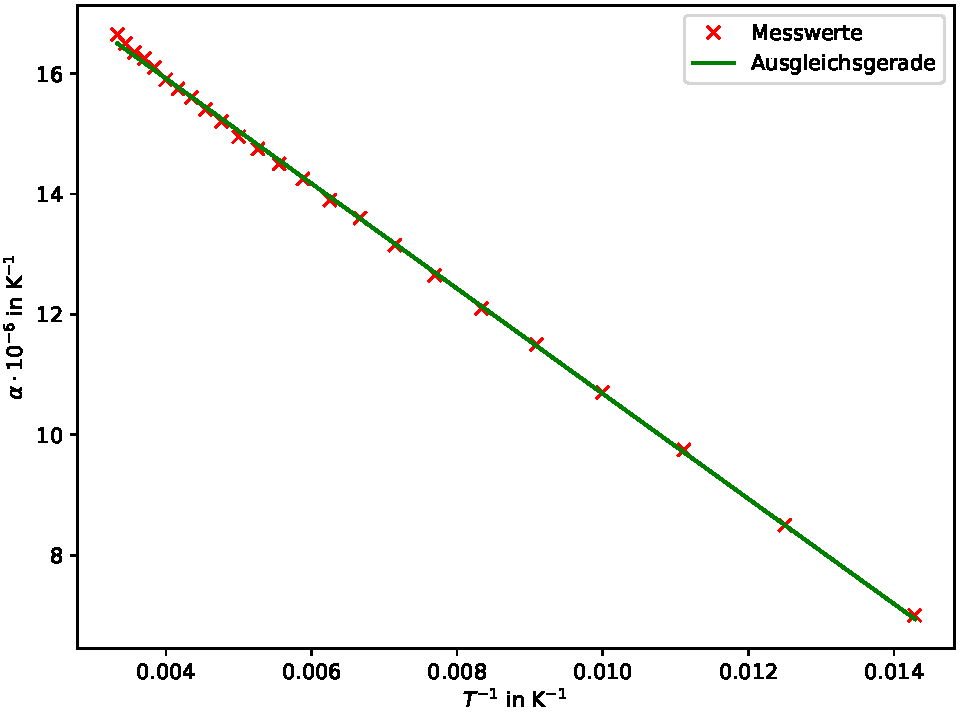
\includegraphics[width=0.9\textwidth]{plots/alphaplot.pdf}
  \caption{Linearer Zusammenhang des Ausdehnungskoeffizienten $\alpha$ gegen die inverse Temperatur $\frac{1}{T}$.}
  \label{fig:alphaplot}
\end{figure}
\clearpage
Die Regression liefert folgende Zahlenwerte für die beiden Parameter $x$ und $y$:
\begin{align*}
	x &=(-873 \pm 4)\cdot 10^{-6}\\
	y &=\SI{19,41 \pm 0,03}{\frac{1}{K}}
\end{align*}
Im Folgenden findet die Berechnung aus den Messwerten der Molwärme bei konstantem Druck $C_P$ und die daraus abgeleitete Molwärme bei konstantem Volumen $C_V$
nach den oben genannten Formeln statt. Alle Messwerte des Versuchs sowie die errechneten Größen $T$, $C_P$ und $C_V$ befinden sich in Tabelle \ref{tab:wertegesamt}.\\
Die nach Formel \ref{eq:cv} berechneten Werte für die molare Wärmekapazität $C_V$ befinden sich in Tabelle \ref{tab:cv}.

\begin{table}[htb]
  \centering
  \caption{Größen zur Bestimmung der molaren Wärmekapazität $C_P$ einer Kupferprobe.}
  \begin{tabular}{S[table-format=2.2,separate-uncertainty,table-figures-uncertainty=1]
                  S[table-format=2.2,separate-uncertainty,table-figures-uncertainty=1]
                  S[table-format=2.2,separate-uncertainty,table-figures-uncertainty=1]
                  S[table-format=2.2,separate-uncertainty,table-figures-uncertainty=1]
                  S[table-format=2.2,separate-uncertainty,table-figures-uncertainty=1]
                  S[table-format=2.2,separate-uncertainty,table-figures-uncertainty=1]}
      \toprule
      {$\delta t$ in \si{\second}} & {$R$ in \si{\ohm}} & {$I$ in \si{\milli\ampere}} & {$U$ in \si{\volt}} & {$T$ in \si{\kelvin}} & {$C_{\mathrm{P}}$ in \si{\joule\per\mol\per\kelvin}} \\
      \midrule
      0(0)  & 22,0(1) & 150,5(1) & 13,27(1) & 81.29(24)&	0(0)\\
      302(3)& 26,2(1) & 153,1(1) & 13,27(1) & 91.21(24)&	11,5(4)\\
      250(3)& 30,0(1) & 154,2(1) & 13,26(1) & 100.22(24)&	10,5(4)\\
      300(3)& 33,3(1) & 154,8(1) & 13,25(1) & 108.07(24)&	14,6(6)\\
      330(3)& 37,0(1) & 164,0(1) & 13,28(1) & 116.92(24)&	15,1(6)\\
      300(3)& 40,8(1) & 173,8(1) & 13,30(1) & 126.04(24)&	14,1(5)\\
      300(3)& 44,4(1) & 170,3(1) & 13,29(1) & 134.71(24)&	14,6(6)\\
      300(3)& 48,0(1) & 178,5(1) & 13,32(1) & 143.43(24)&	15,2(6)\\
      300(3)& 51,7(1) & 181,5(1) & 13,33(1) & 152.41(24)&	15,0(6)\\
      300(3)& 55,4(1) & 186,3(1) & 13,34(1) & 161.44(24)&	15,3(6)\\
      300(3)& 59,3(1) & 186,6(1) & 13,34(1) & 170.99(25)&	14,5(5)\\
      300(3)& 63,1(1) & 186,8(1) & 13,35(1) & 180.34(25)&	14,9(6)\\
      300(3)& 66,7(1) & 186,9(1) & 13,35(1) & 189.23(25)&	15,6(6)\\
      300(3)& 70,3(1) & 187,0(1) & 13,35(1) & 198.16(25)&	15,6(6)\\
      300(3)& 73,8(1) & 188,9(1) & 13,36(1) & 206.87(25)&	16,2(7)\\
      300(3)& 77,5(1) & 189,1(1) & 13,37(1) & 216.12(25)&	15,2(6)\\
      300(3)& 81,1(1) & 189,3(1) & 13,37(1) & 225.15(25)&	15,6(6)\\
      300(3)& 84,3(1) & 189,4(1) & 13,37(1) & 233.21(25)&	17,5(8)\\
      300(3)& 87,6(1) & 189,4(1) & 13,38(1) & 241.54(25)&	17,0(7)\\
      330(3)& 91,0(1) & 189,5(1) & 13,38(1) & 250.16(25)&	18,0(8)\\
      330(3)& 93,6(1) & 189,6(1) & 13,38(1) & 256.78(25)&	23,5(3)\\
      360(3)& 96,3(1) & 189,6(1) & 13,38(1) & 263.66(26)&	24,7(3)\\
      360(3)& 100,5(1) & 189,6(1) & 13,39(1) & 274.41(26)& 15,8(6)\\
      360(3)& 104,8(1) & 189.7(1) & 13,40(1) & 285.47(26)& 15,4(5)\\
      360(3)& 107,8(1) & 189,8(1) & 13,40(1) & 293.21(26)& 22,0(1)\\
			300(3)& 109,9(1) & 189,8(1) & 13,41(1) & 298.64(26)& 26,1(8)\\
      \bottomrule
  \end{tabular}
  \label{tab:wertegesamt}
\end{table}

\begin{table}[htb]
  \centering
  \caption{Wertetabelle für die molare Wärmekapazität bei konstantem Volumen $C_V$.}
  \begin{tabular}{S[table-format=2.2,separate-uncertainty,table-figures-uncertainty=1]
                  S[table-format=2.2,separate-uncertainty,table-figures-uncertainty=2]
                  S[table-format=2.2,separate-uncertainty,table-figures-uncertainty=1]}
      \toprule
    	{$T$ in \si{\kelvin}} & {$\alpha \cdot 10^{-6}$ in \si{\frac{1}{\kelvin}}} & {$C_{\mathrm{V}}$ in \si{\joule\per\mol\per\kelvin}} \\
      \midrule
       91.21(24)&	9,84(6) & 11,5(4)\\
       100.22(24)&	10,70(5) & 10,5(4)\\
       108.07(24)&	11,33(5) & 14,6(6)\\
       116.92(24)&	11,94(5) & 15,1(6)\\
       126.04(24)&	12,48(5) & 14,1(5)\\
       134.71(24)&	12,93(4) & 14,6(6)\\
       143.43(24)&	13,32(4) & 15,2(6)\\
       152.41(24)&	13,68(4) & 15,0(6)\\
       161.44(24)&	14,00(4) & 15,3(6)\\
       170.99(25)&	14,30(4) & 14,5(5)\\
       180.34(25)&	14,57(4) & 14,9(6)\\
       189.23(25)&	14,80(4) & 15,6(6)\\
       198.16(25)&	15,00(4) & 15,6(6)\\
       206.87(25)&	15,19(4) & 15,2(7)\\
       216.12(25)&	15,37(4) & 15,2(6)\\
       225.15(25)&	15,53(4) & 15,6(6)\\
       233.21(25)&	15,67(4) & 17,5(8)\\
       241.54(25)&	15,80(4) & 17,0(7)\\
       250.16(25)&	15,92(4) & 18,0(8)\\
       256.78(25)&	16,01(4) & 23,5(3)\\
       263.66(26)&	16,10(4) & 24,7(3)\\
       274.41(26)& 16,23(4) & 15,8(6)\\
       285.47(26)& 16,35(4) & 15,4(5)\\
       293.21(26)& 16,43(4) & 22,0(1)\\
			 298.64(26)& 16,49(4) & 26,1(8)\\
      \bottomrule
  \end{tabular}
  \label{tab:cv}
\end{table}
\clearpage
Der Zusammenhang zwischen der Temperatur $T$ und der Molwärme $C_V$ ist durch Abbildung \ref{fig:cvplot} dargestellt.
\begin{figure}[H]
  \centering
  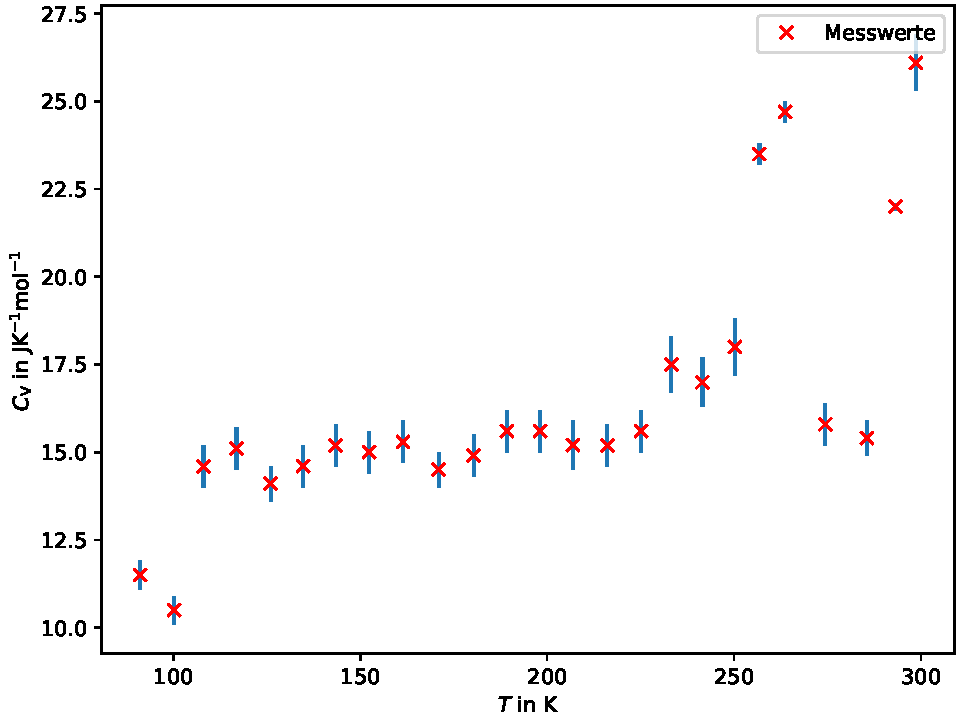
\includegraphics[width=0.9\textwidth]{plots/cvplot.pdf}
  \caption{Zusammenhang zwischen der Temperatur $T$ und der molaren Wärmekapazität $C_V$.}
  \label{fig:cvplot}
\end{figure}
\clearpage
\subsection{Anpassung der Debye-Temperatur}
Für die im Auswertungsteil zuvor bestimmten Wertepaare für $T$ und $C_V$ wird mithilfe von Tabelle 1 aus \cite{anleitung} eine Debye-Temperatur $\theta_D$ approximiert.
Aus der Tabelle abgelesen werden kann der Quotient $\frac{\theta_D}{T}$, wodurch mit Multiplizieren von T die Debye-Temperatur bestimmt werden kann.
Betrachtet werden ausschließlich die Temperaturwerte bis $\SI{170}{K}$.

\begin{table}[htb]
  \centering
  \caption{Wertetabelle für die Bestimmung der Debye-Temperatur $\theta_D$.}
  \begin{tabular}{S[table-format=2.2,separate-uncertainty,table-figures-uncertainty=1]
                  S[table-format=2.2,separate-uncertainty,table-figures-uncertainty=1]
									S[table-format=2.2]
                  S[table-format=2.2,separate-uncertainty,table-figures-uncertainty=1]}
      \toprule
    	{$T$ in \si{\kelvin}} & {$C_{\mathrm{V}}$ in \si{\joule\per\mol\per\kelvin}} & $\frac{\theta_D}{T} $ & {$\theta_D$ in \si{\frac{1}{K}}} \\
      \midrule
       91.21(24)& 11,5(4)& 4,8& 437,8(12)\\
       100.22(24)& 10,5(4)& 4,5& 451,0(11)\\
       108.07(24)& 14,6(6)& 4,3& 464,7(10)\\
       116.92(24)& 15,1(6)& 4,2& 491,1(10)\\
       126.04(24)& 14,1(5)& 4,0& 504,2(10)\\
       134.71(24)& 14,6(6)& 3,9& 525,4(9)\\
       143.43(24)& 15,2(6)& 3,8& 545,0(9)\\
       152.41(24)& 15,0(6)& 3,7& 563,9(9)\\
       161.44(24)& 15,3(6)& 3,6& 581,2(9)\\
       170.99(25)& 14,5(5)& 3,5& 598,5(9)\\
      \bottomrule
  \end{tabular}
  \label{tab:debye}
\end{table}
Der Mittelwert für den experimentell bestimmten Wert ist
\begin{equation*}
	\theta_{D_\text{exp}}= (516,28 \pm 1,86)\si{K}.
\end{equation*}
Nach Formel \ref{eq:debyeintegral} ergibt sich für die Debye-Temperatur unter Berücksichtigung von $v_{\mathrm{l}}=\SI{4.7}{\kilo\metre\per\second}$ und $v_{\mathrm{t}}=\SI{2.26}{\kilo\metre\per\second}$, dass gilt:
\begin{equation}
  \theta_{D_{\text{theo}}}=\frac{\hbar}{k_{\mathrm{B}}}\sqrt[3]{\frac{18\pi^2N_A\rho}{M}\left(v_{\mathrm{l}}^{-3}+2v_{\mathrm{t}}^{-3}\right)^{-1}}.
\end{equation}
Als so theoretisch bestimmter Wert ergibt sich eine Debye-Temperatur von
\begin{equation*}
	\theta_{D_\text{theo}}=\SI{332,5}{\kelvin}.
\end{equation*}

Für die Debye-Frequenzen folgen aus
\begin{equation}
	\omega_D = \frac{k_B \theta_D}{\hbar}
\end{equation}
\begin{align*}
	\omega_{exp} &= (67,59 \pm 0,26)\si{THz}\\
	\omega_{theo} &= \SI{43,53}{THz}.
\end{align*}
